\section{SVT Cooling}

All the GUIs shown below are accessed through the \textbf{Devices} menu in \textbf{hps\_epics}.

\begin{figure*}[!ht]
    \begin{center}
        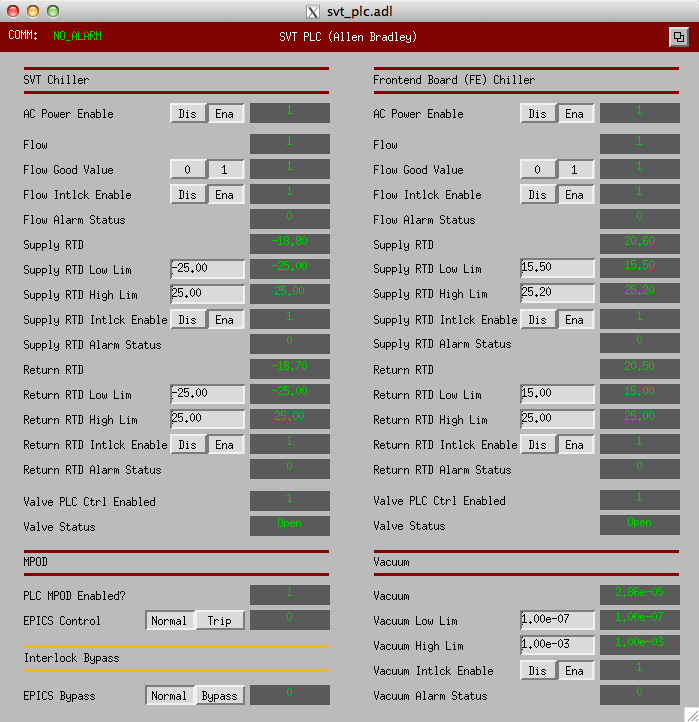
\includegraphics[width=0.5\textwidth]{svt_plc.png}
        \caption{SVT PLC GUI, accessed through the \textbf{Devices} menu in \textbf{hps\_epics}.}
        \label{fig:ctrl_cooling_plc}
    \end{center}
\end{figure*}

\begin{figure*}[!ht]
    \begin{center}
        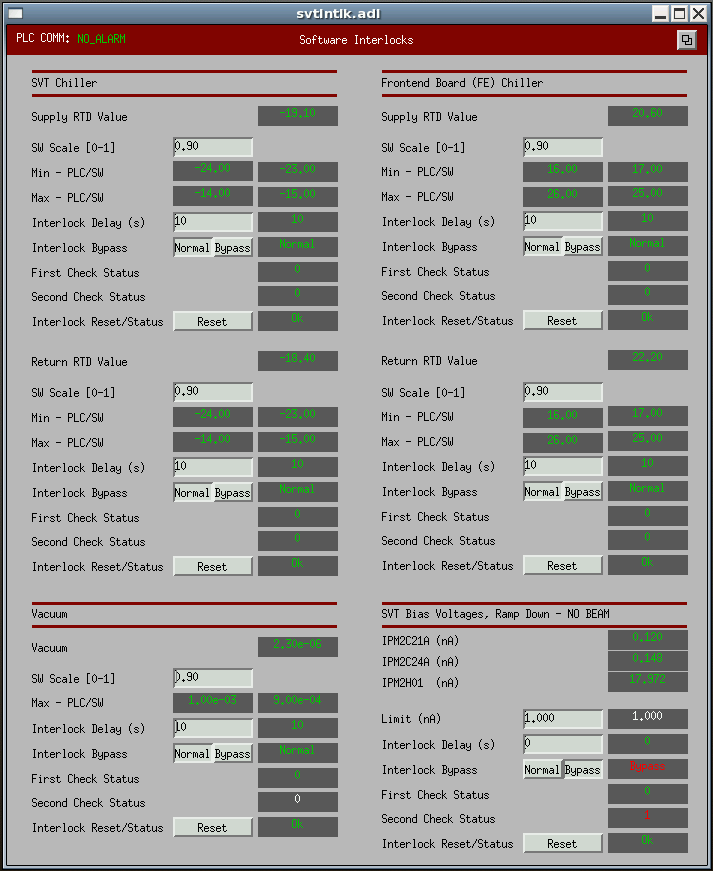
\includegraphics[width=0.4\textwidth]{svt_softinterlocks.png}
        \caption{SVT software interlocks GUI, accessed through the \textbf{Devices} menu in \textbf{hps\_epics}.}
        \label{fig:ctrl_cooling_softinterlocks}
    \end{center}
\end{figure*}

\begin{figure*}[!ht]
    \begin{center}
        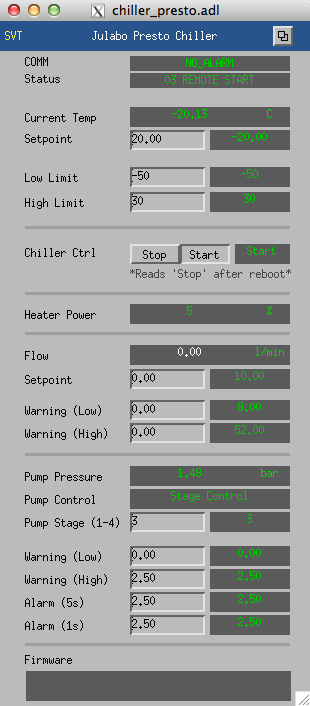
\includegraphics[width=4cm]{figures/svt_svtChiller.png}
        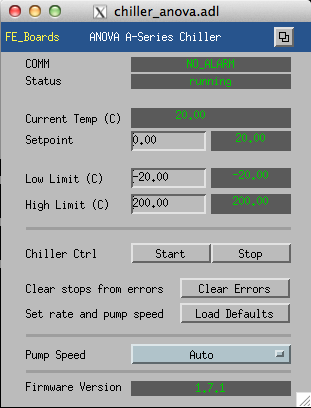
\includegraphics[width=0.3\textwidth]{figures/svt_febChiller.png}
        \caption{SVT (left) and FEB (right) chiller GUIs, accessed through the \textbf{Devices} menu in \textbf{hps\_epics}.}
        \label{fig:ctrl_cooling_chillers}
    \end{center}
\end{figure*}

\begin{table}[h]
\begin{center}
\begin{tabular}{|l|l|l|}
\hline
Parameter & SVT warm & SVT cold \\
\hline
SVT chiller setpoint (C) & 17 & -20 \\
SVT RTD alarms (C) & 15/16/18/19 & -22/-21/-17/-16 \\
SVT RTD PLC limits (C) & bypassed & -24/-14 \\
FEB chiller setpoint (C) & 20 & 20 \\
\hline
\end{tabular}
\end{center}
\caption{SVT cooling settings.}
\end{table}

Also, there is a webcam (cctv7) pointed at the SVT chiller screen. The webcam can be set to e-mail a snapshot every 24 hours.

Any major (red) ALH alarm under the ``SVT/COOLING'' group will send an e-mail alert.
